\documentclass{article}
\usepackage{hyperref}
\usepackage[T1]{fontenc}
\usepackage[polish]{babel}
\usepackage[utf8]{inputenc}
\usepackage{lmodern}
\selectlanguage{polish}
\usepackage{indentfirst} 
\setlength
\parindent{24pt}
\usepackage{multirow}
\usepackage{siunitx}
\usepackage{graphicx}
\usepackage{natbib}
\usepackage{amsmath}
\usepackage{latexsym}
\pagenumbering{arabic}

\setlength\parindent{0pt}

\usepackage{geometry}
\newgeometry{vmargin={22mm}, hmargin={22mm,30mm}}




\renewcommand{\labelenumi}{\alph{enumi}.}
\title{Projekt zespołowy:\\Django Boys\\} % Title

\author{} 
\date{}



\begin{document}
\title{
\includegraphics[scale=0.7]{UG.jpg}\\[2cm]{Projekt zespołowy:\\Django Boys \\[10cm] \href{https://github.com/DjangoBo/Python}{GitHub link}}}
\maketitle

\begin{center}
\begin{tabular}{l r}
Data oddania & 20.01.2020 \\ 
\end{tabular}
\end{center}


\newpage
\Large

\tableofcontents



\newpage


\section{Przebieg prac}

\subsection{Stworzenie drużyny i pomysł}
\parindent24pt Na początku nasza grupa liczyła dwie osoby. Na podstawie języków używanych na innych zajęciach wybraliśmy pythona jako narzędzie którego chcielibyśmy się nauczyć. Wiedząc, że na potrzeby inteligencji obliczeniowej będziemy musieli mauczyć się podstaw języka, jako projekt postanowiliśmy wybrać framework do pythona. Padło na django. Po rozpadzie jednej z ekip dołączyła do nas trzecia osoba i tak wyklarował się skład Django Boys. Postanowiliśmy, że zrobimy sklep internetowy sprzedający rzeczy z dzikiego zachodu, nawiązując do filmu Quentina Tarantino.
\subsection{Początek pracy}
\parindent24pt Pierwszym zadaniem było przygotowanie harmonogramu (dostępny w repozytorium GitHub). Jako, że zaczynaliśmy przygodę z programowaniem prawie od zera postanowiliśmy się posiłkować książką 'Django 2' autorstwa Antonio Melé. Ustaliliśmy, że pythona nauczymy się skupiając się na innych przedmiotach, więc przy okazji wykonamy część projektu zespołowego. \par Po zakupie książki mieliśmy wrażenie, że już coś zrobiliśmy i wtedy zaczęły się opóźnienia w stosunku do założonego harmonogramu. Założyliśmy wtedy czat na messengerze, aby usprawnić komunikację, jednak przez większą część semestru mało z niego korzystaliśmy.
\subsection{Praca z pythonem}
\par Każdy z nas osobno nauczył się podstaw pythona takich jak pętle, tablice jedno i wielowymiarowe, obsługi paczek takich jak: matplotlib, numpy, czy pandas. Poznaliśmy również podstawy algorytmów genetycznych, machine learningu i analizy tekstu. Robiliśmy to jednak całkowicie osobno bez współpracy ani kontaktu, przez co minęliśmy się trochę z założeniami projektu zespołowego. \par Na przedmiocie 'Zaawansowane języki programowania' zajęliśmy się refaktoryzacją \href{https://github.com/emilybache/GildedRose-Refactoring-Kata}{Gilded Rose Kata}. Każdy z nas, musiał samemu na podstawie wykładu dokonać refaktoryzacji kodu. Wszyscy jako język wybraliśmy również pythona. Refaktoryzacja udała się każdemu z nas, jednak znów robiliśmy to całkowicie osobno.

\subsection{Praca z django}
\par Nasza praca z django opóźniła się znacznie w stosunku do harmonogramu. Zaczęliśmy się aktywniej komunikować odnośnie projektu dopiero 8 stycznia, co pokazuje jak dużo czasu zmarnowaliśmy. Pierwsza aplikacja bloga powstała dość sprawnie jednak i tak było to około miesięczne opóźnienie względem planów. \par Gdy już każdy z nas miał jakiekolwiek pojęcie na temat django zaczęliśmy próbować tworzyć nasz sklep. Powoli zaczęliśmy dodawać małe funkcjonalności. Na koniec zaczęliśmy tworzyć wspólny sklep, który finalnie działał co zakończyło nasz projekt. Na sam koniec postanowiliśmy dodać ciekawą opcję jaką jest generowanie rachunków w formacie PDF, co zakończyło ostatecznie pisanie kodu.



\newpage

\section{Projekt}

\subsection{Python}
\par Programy dostępne w repozytorium jako część związana z nauką pythona, to program przechodzący labirynt używając algorytmu genetycznego i prosta gra napisana przy pomocy PyGame.\par Labirynth.py napisany jest bez użycia bibliotek używanych do uczenia maszynowego. Algorytm jest napisany samodzielnie i uwzględnia zarówno mutacje, jak i elityzm, co zwiększa jego skuteczność. wyniki są przedstawione za pomocą biblioteki matplotlib.
\begin{center}
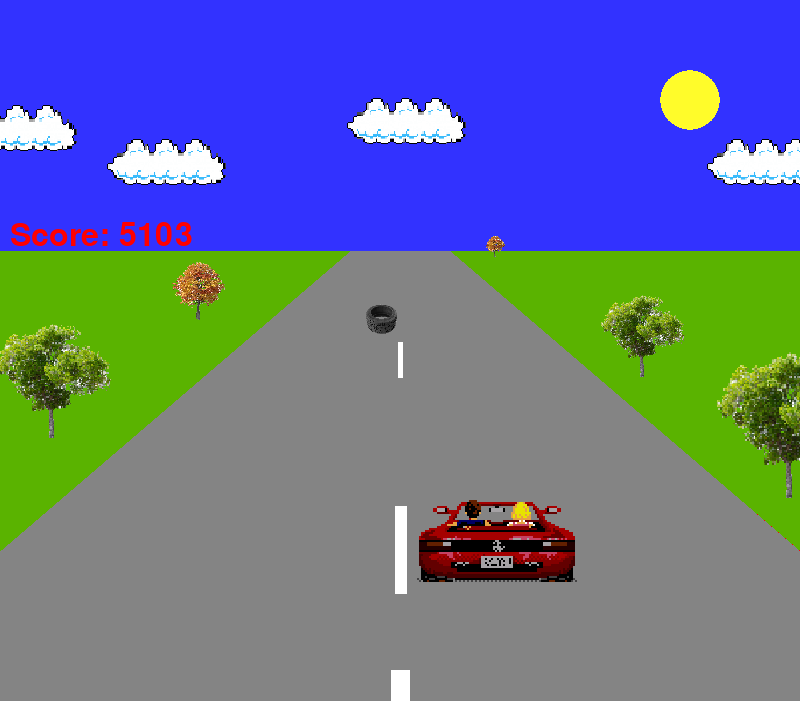
\includegraphics[scale=0.35]{pygame.png}\\
Screen z gry w pygame.
\end{center}

\begin{center}
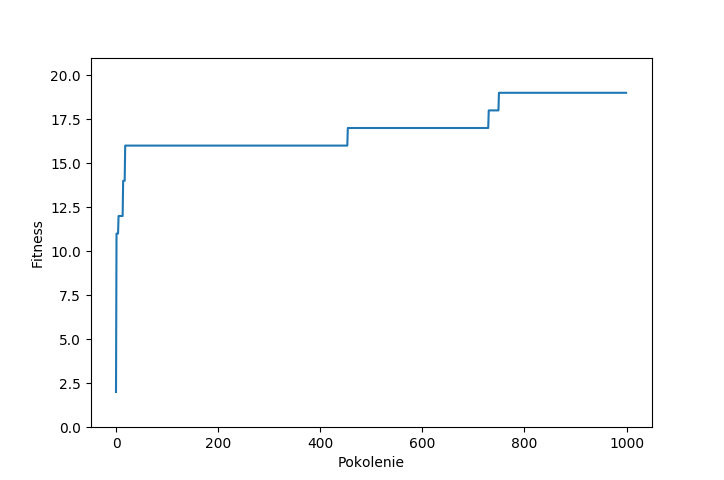
\includegraphics[scale=0.69]{Figure_1.png}\\
Ciekawe przejście labiryntu, w którym widać skoki funkcji fitnes w późnych pokoleniach. Spowodowane są one mutacjami.
\end{center}

\subsection{Django}
\subsubsection{Blog}
Blog, który wykonaliśmy jest prosty i nie posiada żadnych podstron. Posty dodawać można w panelu administracyjnym. Panel ten umożliwia wybranie godziny publikacji innej, niż godzina wpisu. Posty na stronie wyświetlane są w poprawnej kolejności razem z tytułem i datą. Na prawym panelu znalazło się okienko 'O nas'.
\\[2cm]
\begin{center}
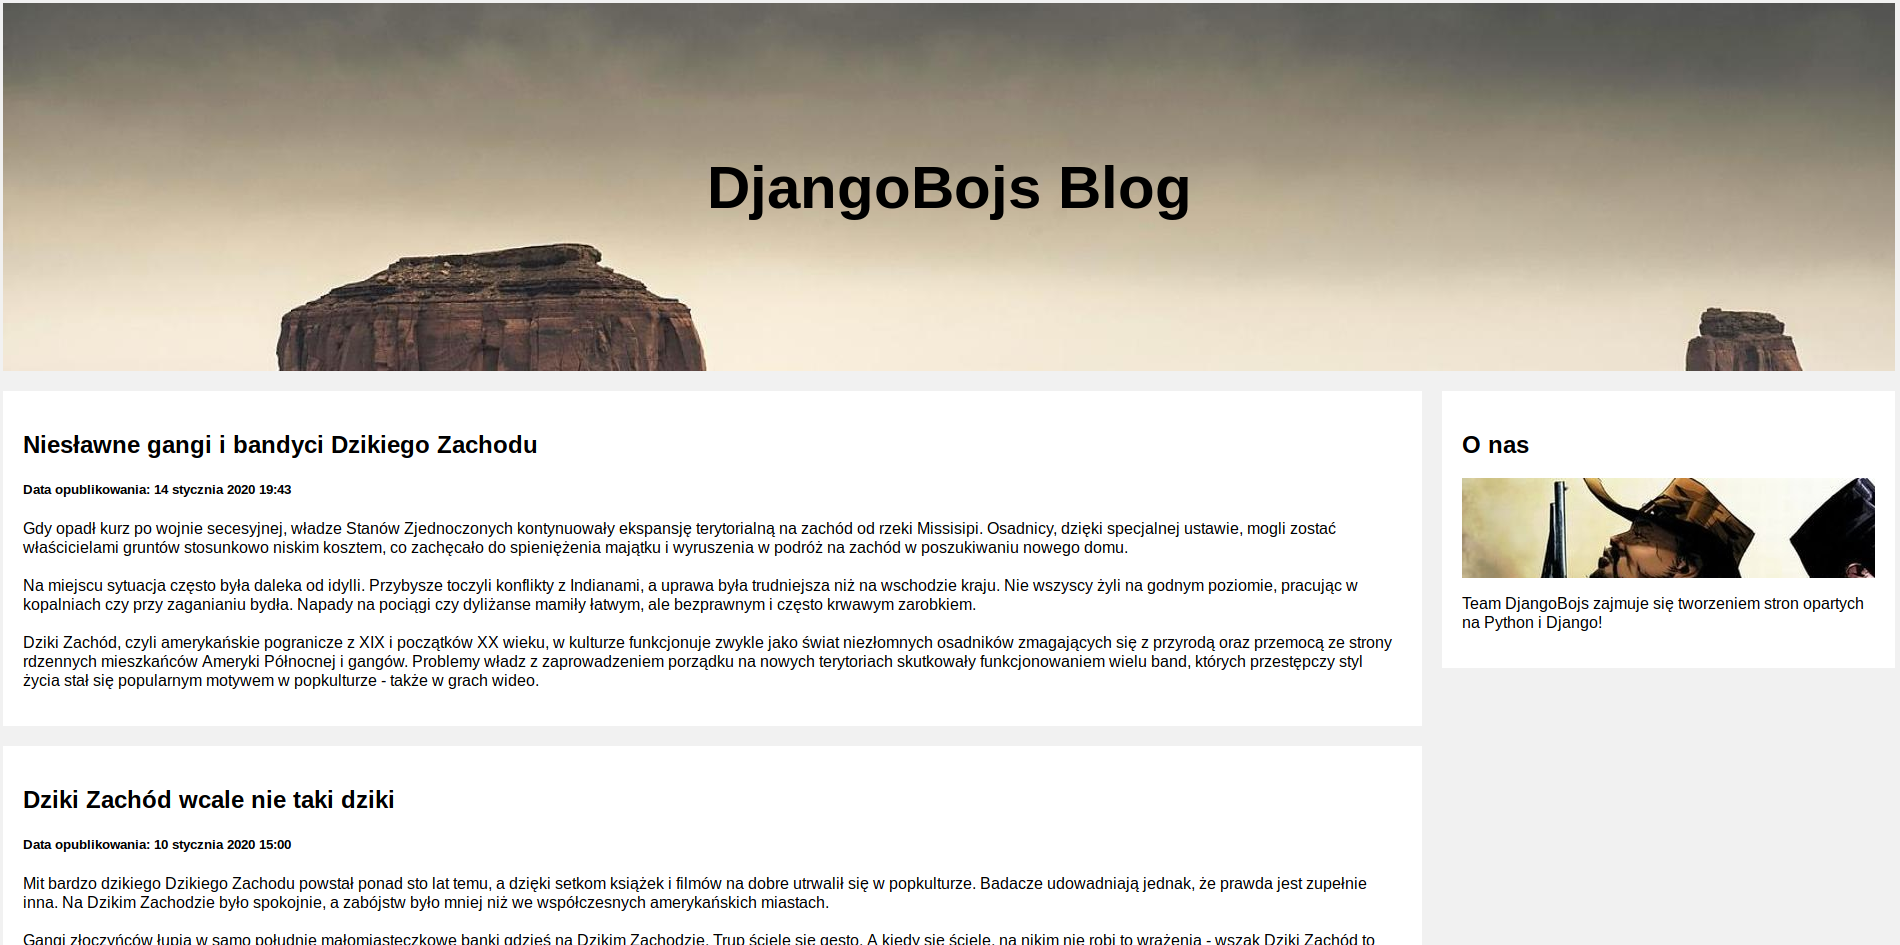
\includegraphics[scale=0.35]{blog.png}\\
Wygląd bloga.
\end{center}

\newpage

\subsubsection{Sklep}
\par Sklep został ukończony zdecydowanie zbyt późno, aby można go było ulepszyć. Gdyby nie zbyt późne podjęcie prac w django bylibyśmy w stanie stworzyć bardziej rozwinięty projekt. Jednak oddajemy prostą ale sprawną wersję, w której na koniec postanowiliśmy dodać generator rachunków w formacie PDF. Oto lista funkcjonalności naszego sklepu:
\begin{itemize}
\item dodawanie produktów i kategorii z poziomu witryny administracyjnej
\item wyświetlanie produktów według kategorii
\item wyświetlanie szczegółowych stron produktów ze zdjęciami
\item działający koszyk i składanie zamówień
\item możliwość zmiany ilości towaru tuż przed dokonamien zamównienia
\item wyświetlanie szczegółów zamówień w witrynie administracyjnej
\item Generowanie rachunków w formacie PDF
\end{itemize}

\begin{center}

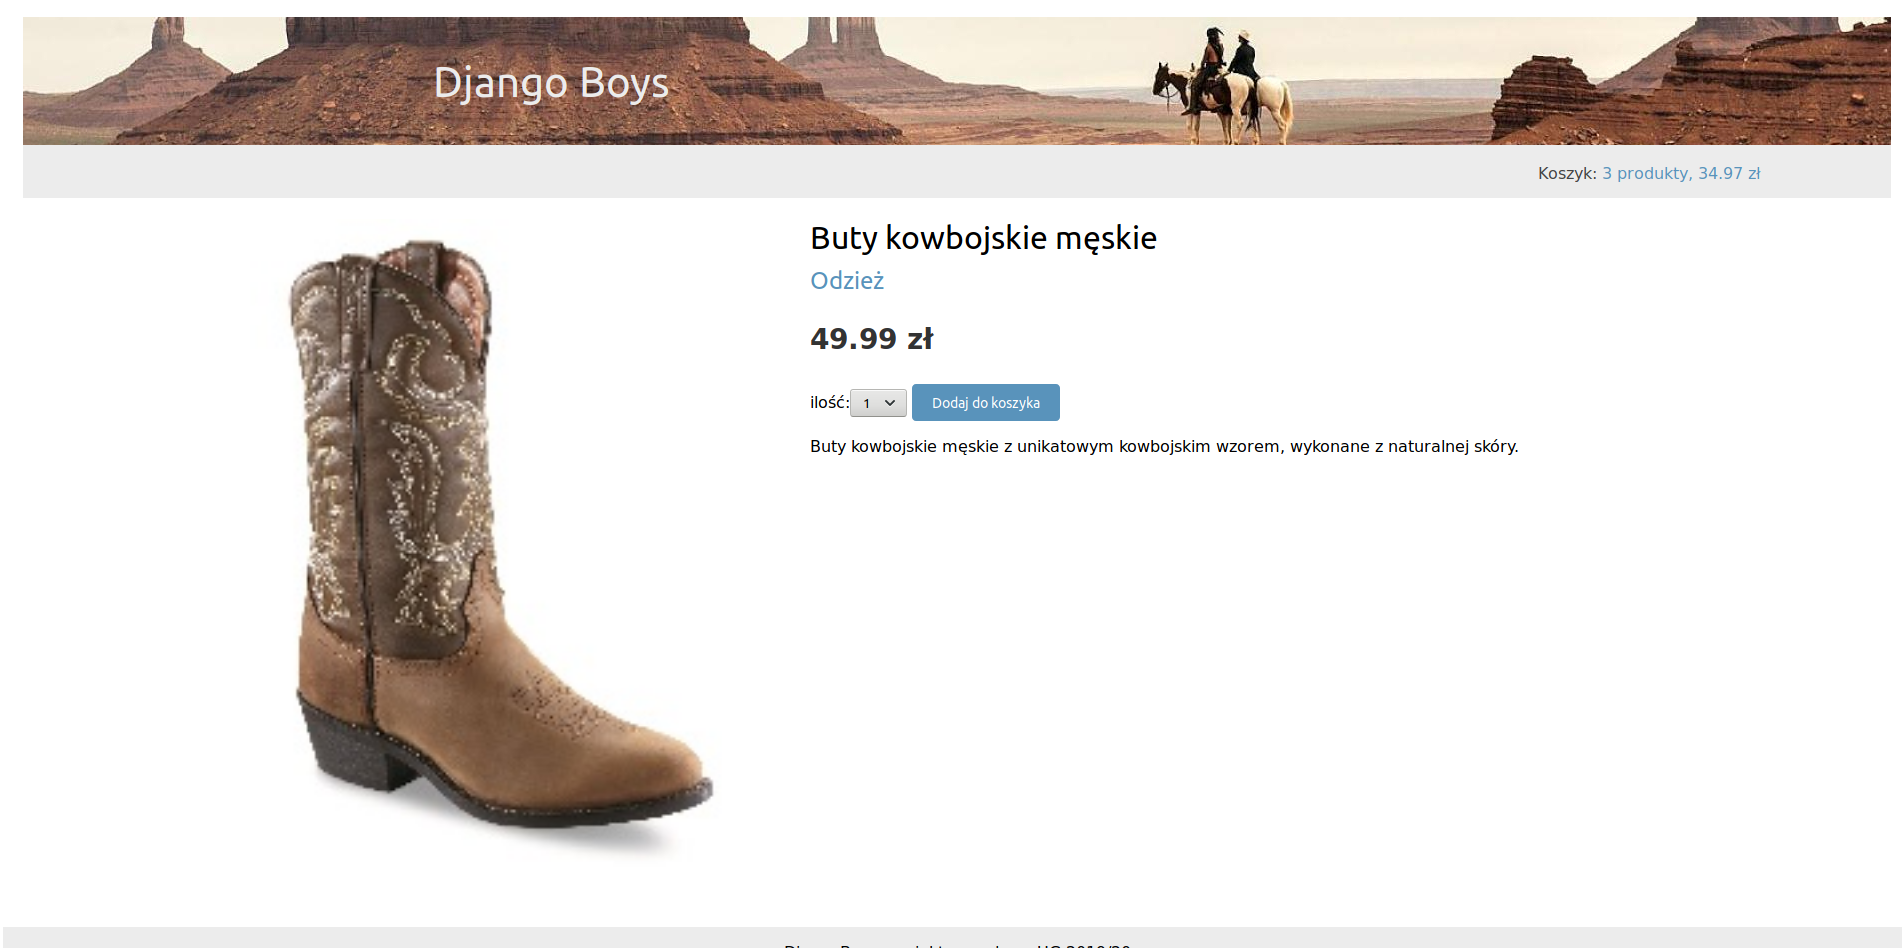
\includegraphics[scale=0.35]{szczegoly.png}\\
Wygląd strony szczegółowej produktu.
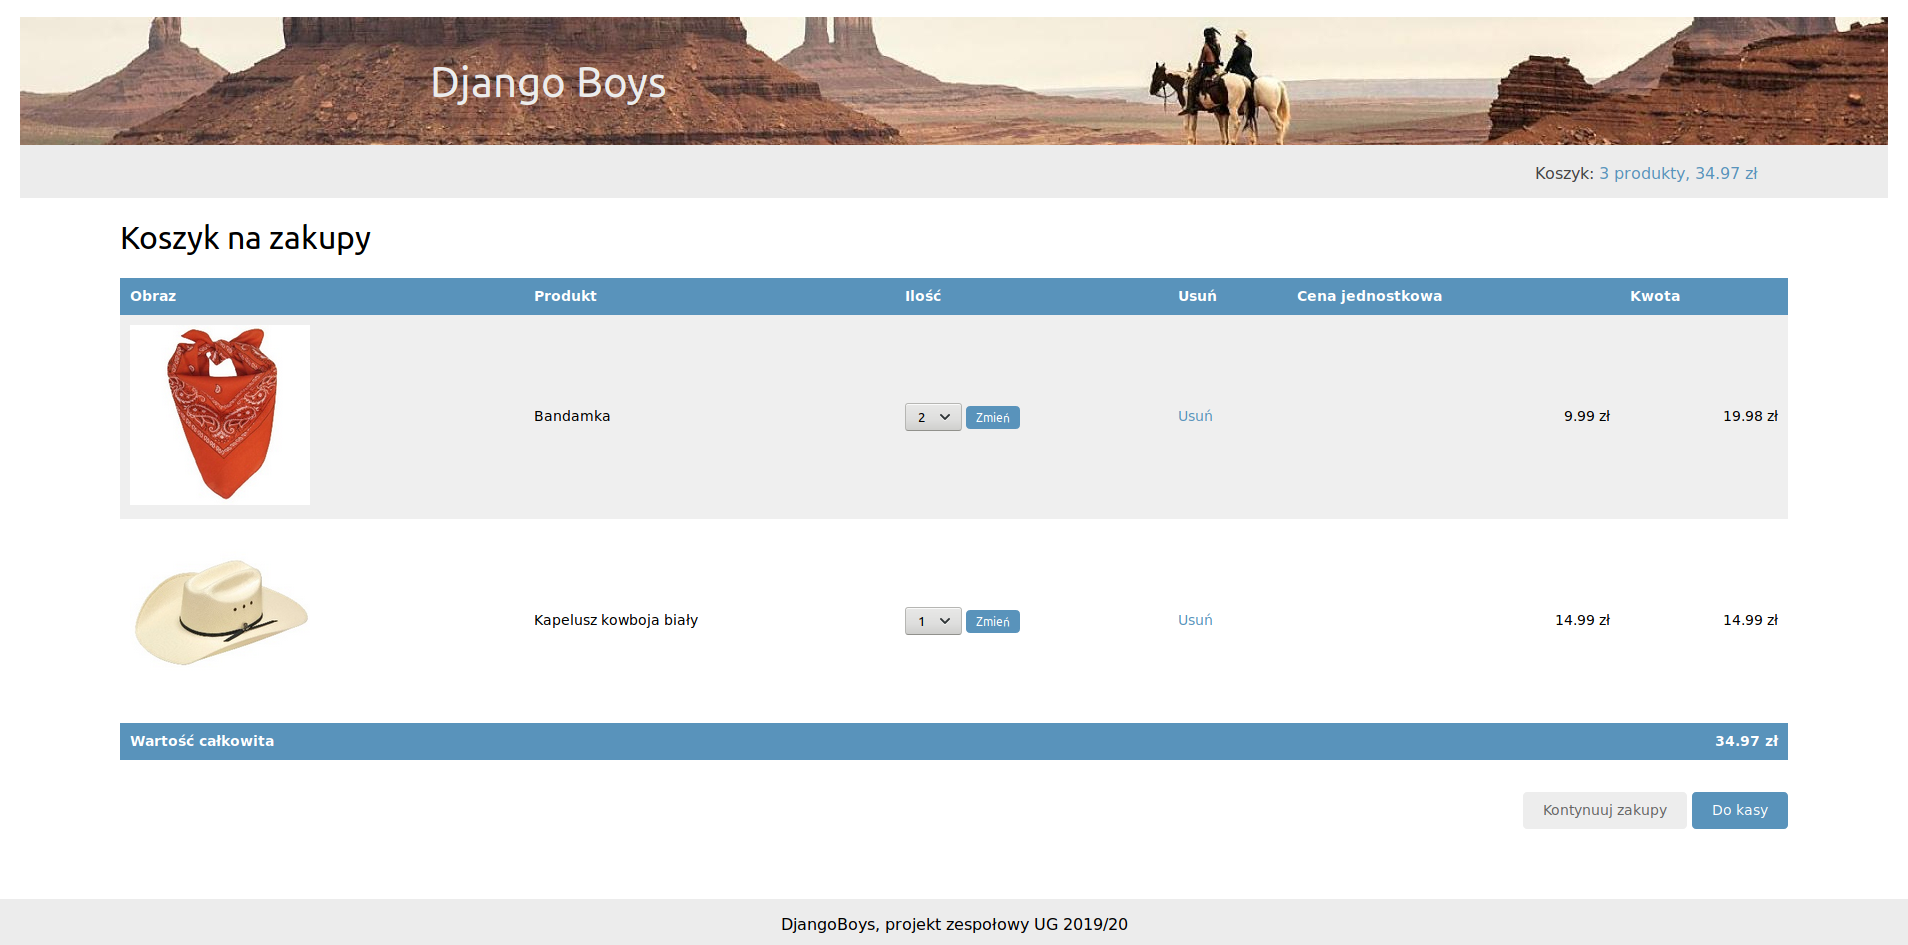
\includegraphics[scale=0.35]{koszyk.png}\\
Wygląd koszyka zakupów.\\[2cm]
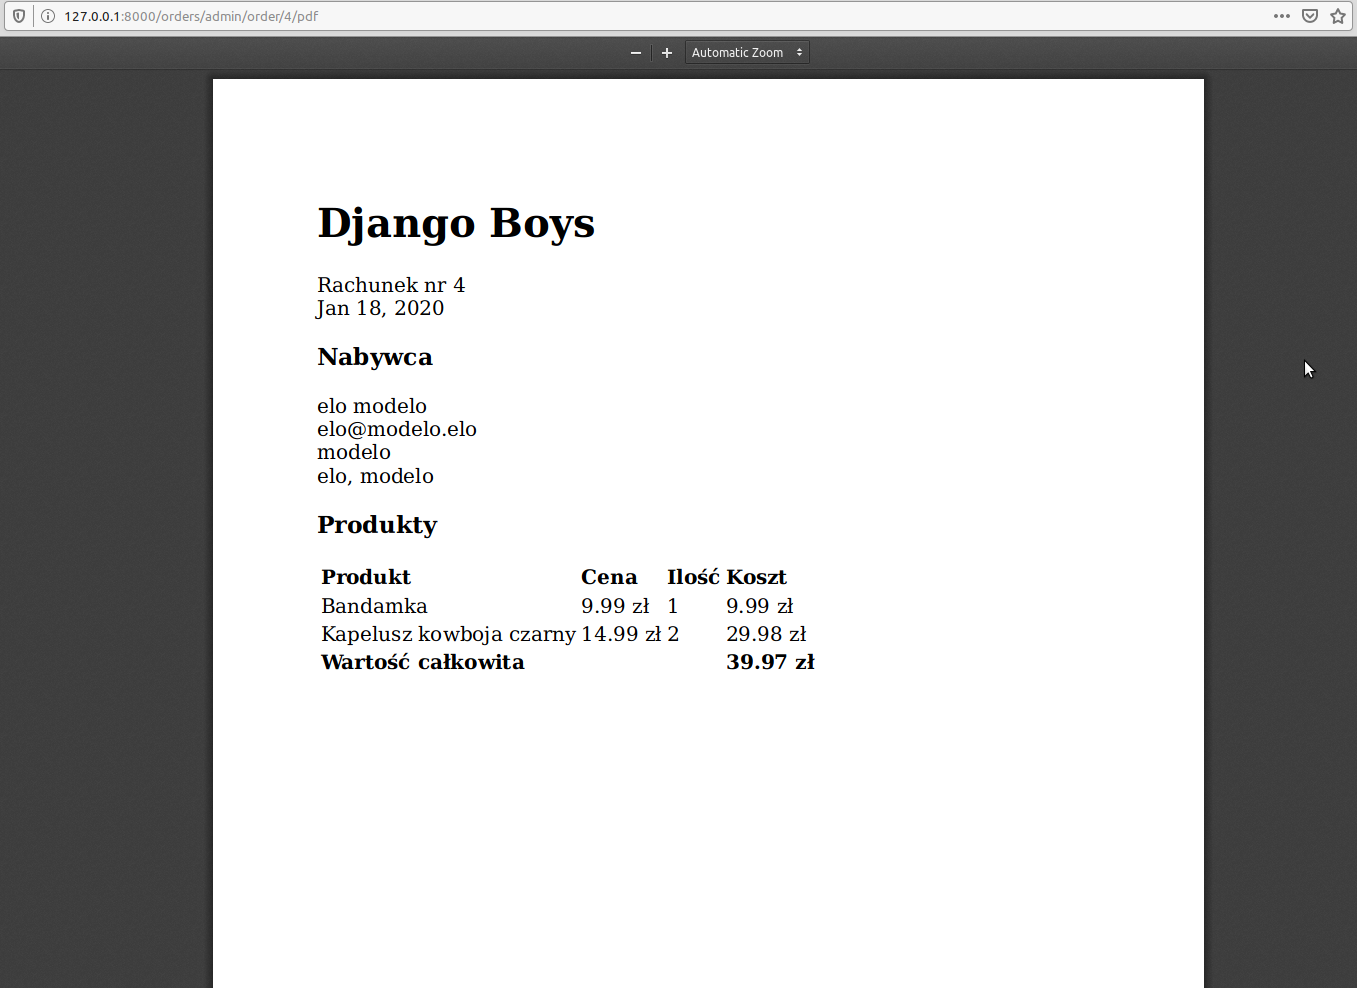
\includegraphics[scale=0.35]{pdf.png}\\
Wygenerowany rachunek PDF.
\end{center}




\newpage
\section{Oceny wewnątrz grupy}
\subsection{Ocena zespołu według PM}
\par Projekt zakończył się powodzeniem, więc ocena zespołu jest pozytywna. Każdy z nas się czegoś nauczył i poszerzył swoją wiedzę.
\subsubsection{Ocena Pawła} \par Na starcie miał najmniejszą styczność z programowaniem z całego zespołu, a pythona poznawał od zera. Od początku widać było zaangażowanie i chęć ukończenia projektu. To jego wersja bloga okazała się najatrakcyjniejszą wizualnie i została dołączona do repozytorium. Nie opanował w pełni obsługi gita, przez co programy wrzucał na własne repozytorium. W grudniu zgłaszał, że jest zapracowany, co pokazuje szacunek do reszty zespołu. Pomagał w tworzeniu sklepu wyszukując grafiki, teksty, jak i tutoriale które pomogły nam ukończyć projekt.
\subsubsection{Ocena Władysława}
Dołączył do zespołu jako ostatni, gdy temat już był wybrany. Więc mógł mu nie podpasować. Jego mocniejszą stroną jest programowanie w pythonie niż przy pomocy django. Udzielał się głównie na początku prac. Również stworzył własną wersję bloga.
\newpage
\subsection{Ocena PM według członków zespołu}
Oceny są skopiowane prosto od autorów, PM wrzucił je tylko do sprawozdania.
\subsubsection{Ocena Pawła}
\par Lokomotywą naszego zespołu był Team Leader. Od początku przejął stery nad projektem, wydawał zadania i polecenia. Starał się nas motywować i popędzał do pracy. W każdym etapie wspólnej realizacji projektu mogłem na niego liczyć, starał się pomagać. Szanował czas pozostałych osób w grupie, dobrze organizował czas. W mojej ocenie ciężko mu było wywrzeć na nas presję, stąd powstałe opóźnienia. Myślę, że był dobrym Team Leaderem – nie podejmował decyzji sam ale był otwarty na nasze propozycje.
\subsubsection{Ocena Władysława}
Praca w zespole była bardzo przyjemna i produktywna. Byl opracowany projekt sklepu internetowego i zadanie to zostało pomyślnie ukończone. Każdy z nas otrzymał coś użytecznego i znaczącego z tego projektu.

\newpage
\section{Subiektywne posdumowanie projektu przez PM}
Wybraliśmy projekt zbyt ogólny, co utrudniło współpracę, ponieważ nad samą nauką języka łatwo pracować samemu.
\par Zakup książki nie powinien być traktowany jako pierwszy krok, ponieważ jest do złudne poczucie zrobienia 'czegoś', zdecydowanie lepszym pierwszym krokiem jest skończony pierwszy rozdział. \par Powinniśmy wziąć do grupy osobę, która ma szersze pojęcie na temat pracy zespołowej w IT, aby nas koordynowała. Wiem jednak, że jest to trudne, ponieważ na pierwszych zajęciach mało o sobie wiemy nawzajem.
\par Jako PM powinienem zdecydowanie bardziej starać się przestrzegać harmonogramu i wymagać tego od zespołu. Powinienem być również bardziej konsekwentny i wymagający, gdy czegoś oczekuję i daję na to termin wykonania. \par Messenger nie jest najlepszą formą komunikacji w zespole, zaproponowałem również discord, który możliwe, że byłby lepszą opcją, jednak bez pozytywnego odzewu.
\par Fakt, że udało nam się ukończyć projekt mimo późnego startu cieszy. Wraz z zespołem jesteśmy świadomi naszych błędów i spróbujemy uniknąć ich w przyszłości. Wszyscy wyciągneliśmy z tego projektu lekcję.


\end{document}